\documentclass{article}[18pt]
\ProvidesPackage{format}
%Page setup
\usepackage[utf8]{inputenc}
\usepackage[margin=0.7in]{geometry}
\usepackage{parselines} 
\usepackage[english]{babel}
\usepackage{fancyhdr}
\usepackage{titlesec}
\hyphenpenalty=10000

\pagestyle{fancy}
\fancyhf{}
\rhead{Sam Robbins}
\rfoot{Page \thepage}

%Characters
\usepackage{amsmath}
\usepackage{amssymb}
\usepackage{gensymb}
\newcommand{\R}{\mathbb{R}}

%Diagrams
\usepackage{pgfplots}
\usepackage{graphicx}
\usepackage{tabularx}
\usepackage{relsize}
\pgfplotsset{width=10cm,compat=1.9}
\usepackage{float}

%Length Setting
\titlespacing\section{0pt}{14pt plus 4pt minus 2pt}{0pt plus 2pt minus 2pt}
\newlength\tindent
\setlength{\tindent}{\parindent}
\setlength{\parindent}{0pt}
\renewcommand{\indent}{\hspace*{\tindent}}

%Programming Font
\usepackage{courier}
\usepackage{listings}
\usepackage{pxfonts}

%Lists
\usepackage{enumerate}
\usepackage{enumitem}

% Networks Macro
\usepackage{tikz}


% Commands for files converted using pandoc
\providecommand{\tightlist}{%
	\setlength{\itemsep}{0pt}\setlength{\parskip}{0pt}}
\usepackage{hyperref}

% Get nice commands for floor and ceil
\usepackage{mathtools}
\DeclarePairedDelimiter{\ceil}{\lceil}{\rceil}
\DeclarePairedDelimiter{\floor}{\lfloor}{\rfloor}

% Allow itemize to go up to 20 levels deep (just change the number if you need more you madman)
\usepackage{enumitem}
\setlistdepth{20}
\renewlist{itemize}{itemize}{20}

% initially, use dots for all levels
\setlist[itemize]{label=$\cdot$}

% customize the first 3 levels
\setlist[itemize,1]{label=\textbullet}
\setlist[itemize,2]{label=--}
\setlist[itemize,3]{label=*}

% Definition and Important Stuff
% Important stuff
\usepackage[framemethod=TikZ]{mdframed}

\newcounter{theo}[section]\setcounter{theo}{0}
\renewcommand{\thetheo}{\arabic{section}.\arabic{theo}}
\newenvironment{important}[1][]{%
	\refstepcounter{theo}%
	\ifstrempty{#1}%
	{\mdfsetup{%
			frametitle={%
				\tikz[baseline=(current bounding box.east),outer sep=0pt]
				\node[anchor=east,rectangle,fill=red!50]
				{\strut Important};}}
	}%
	{\mdfsetup{%
			frametitle={%
				\tikz[baseline=(current bounding box.east),outer sep=0pt]
				\node[anchor=east,rectangle,fill=red!50]
				{\strut Important:~#1};}}%
	}%
	\mdfsetup{innertopmargin=10pt,linecolor=red!50,%
		linewidth=2pt,topline=true,%
		frametitleaboveskip=\dimexpr-\ht\strutbox\relax
	}
	\begin{mdframed}[]\relax%
		\centering
		}{\end{mdframed}}



\newcounter{lem}[section]\setcounter{lem}{0}
\renewcommand{\thelem}{\arabic{section}.\arabic{lem}}
\newenvironment{defin}[1][]{%
	\refstepcounter{lem}%
	\ifstrempty{#1}%
	{\mdfsetup{%
			frametitle={%
				\tikz[baseline=(current bounding box.east),outer sep=0pt]
				\node[anchor=east,rectangle,fill=blue!20]
				{\strut Definition};}}
	}%
	{\mdfsetup{%
			frametitle={%
				\tikz[baseline=(current bounding box.east),outer sep=0pt]
				\node[anchor=east,rectangle,fill=blue!20]
				{\strut Definition:~#1};}}%
	}%
	\mdfsetup{innertopmargin=10pt,linecolor=blue!20,%
		linewidth=2pt,topline=true,%
		frametitleaboveskip=\dimexpr-\ht\strutbox\relax
	}
	\begin{mdframed}[]\relax%
		\centering
		}{\end{mdframed}}
\lhead{CT}
\usepackage{minted}
\usepackage{listings}
\usepackage{mathtools}
\DeclarePairedDelimiter{\ceil}{\lceil}{\rceil}
\begin{document}
\begin{center}
\underline{\Large How might we develop algorithms to solve fundamental problems?}
\end{center}
\section{Describing Algorithms}
\begin{itemize}
	\item Try to develop a more precise language to describe algorithms - pseudo code
\end{itemize}
\section{The first algorithm}
\begin{itemize}
	\item Euclid's algorithm
\end{itemize}
\begin{minted}{python}
if n==0:
	output m
else:
	set m1=n and n1= m mod n
	set m=m1 and n=n1 and repeat the algorithm
\end{minted}
\subsection{Issues from Euclid's algorithm}
\begin{itemize}
	\item Does it always calculate the GCD?
	\item Does it halt?
	\item Is the implementation correct?
	\item Is it efficient
	\begin{itemize}
		\item Computation time
		\item Memory Usage
	\end{itemize}
\end{itemize}
\section{More on pseudo-code}
\begin{itemize}
	\item It is a list of instructions for menial tasks
	\item Can change the information in "pigeon holes"
	\item Ask yes no questions through flow control
\end{itemize}
\section{Recursion}
\begin{itemize}
	\item The idea of "stop what you are doing and repeat from the start on different data; when you are done, pick up where you left off"
	\item The algorithm is calling itself
\end{itemize}
\begin{minted}{python}
algorithm: Euclid(m,n)
if n==0:
	output m
else:
	set m=n and n=m mod n
	Euclid(m,n)
\end{minted}
\subsection{Non recursive euclid}
Assume that $m\geq n\geq 0$ are non negative integers
\begin{minted}{python}
while n!=0:	
	m=m-n
	if n>m:
		swap m and n
output m
\end{minted}
\subsection{Comparison}
\begin{itemize}
	\item One will have more steps than the other, depends on the algorithm
	\item Compare memory efficiency
\end{itemize}
\section{Yet more on pseudo-code}
\begin{itemize}
	\item Pseudo-code needs to tell us what out inputs, outputs and stored data are
	\item 
\end{itemize}
Fundamental sorting problem:
\begin{itemize}
	\item instance: a list of n integers
	\item output: a list sorted into ascending order
\end{itemize}
\section{Bubble Sort}
Assume that our input is always a list A of n integers, held in cells A[0], A[1], . . . , A[n - 1], or A[0..n - 1] for short, and our aim is to output this list of numbers sorted into ascending order.
\begin{itemize}
	\item The algorithm Bubble-sort repeatedly ‘passes’ through the input list of
	numbers, comparing and swapping adjacent numbers in the list.
	\item In a pass through the input list, consecutive pairs of numbers are compared
	in turn, and these numbers are swapped (in their locations) if
	the first number is greater than the second.
	\item If a swap has been made in a pass through the list then another pass
	is undertaken, otherwise the algorithm halts
\end{itemize}
\begin{lstlisting}[tabsize=4]
change = true
WHILE change == true:
	change = false
	i = 0
	WHILE i < n - 1:
		IF A[i] > A[i + 1]:
			swap A[i] and A[i + 1]
			change = true
		i = i + 1
output A
\end{lstlisting}
\subsection{An execution of Bubble Sort}
\begin{itemize}
	\item During pass 0, bubble sort finds the largest element in the list and puts it in its place
	\item After that it does a bubble sort on the first n-1 elements of the list
	\item This suggests proof by induction
	\item To optimise the number of algorithmic operations, think about this and notice that the previously placed element is still compared, even though the answer is known, so the comparison is unneeded
\end{itemize}
\begin{lstlisting}[tabsize=4,escapechar={£}]
change = true £\textcolor{red}{and pass=0}£
WHILE change == true:
	change = false
	i = 0
	£\textcolor{red}{WHILE i < n - 1 - pass:}£
		IF A[i] > A[i + 1]:
			swap A[i] and A[i + 1]
			change = true
		i = i + 1
	£\textcolor{red}{pass = pass +1}£
output A
\end{lstlisting}
\section{Selection Sort}
There are lots of ways to solve our sorting problem, here is how to do selection sort
\begin{itemize}
	\item Take the number a[0] and store it as x
	\item pass 0: compare x with the numbers in A[1], A[2], . . . , A[n - 1] in turn,
	always keeping the smaller number in x and the larger number in the
	list cell;
	\item put the resulting number x into A[0];
	\item take the number in A[1] and store it as x;
	\item pass 1: compare x with the numbers in A[2], A[3], . . . , A[n - 1] in turn,
	always keeping the smaller number in x and the larger number in the
	list cell;
	\item put the resulting number x into A[1];
	\item take the number in A[2] and store it as x;
	\item pass 2: compare x with the numbers in A[3], A[4], . . . , A[n - 1] in turn,
	always keeping the smaller number in x and the larger number in the
	list cell;
	\item put the resulting number x into A[2];
\end{itemize}
\subsection{Pseudo Code}
\begin{lstlisting}[tabsize=4,mathescape]
pass = 0 
WHILE pass < n - 1:
	x = A[pass]
	i = pass + 1 
	WHILE i $\leqslant$ n - 1: 
		IF A[i] $<$ x:
			swap x and A[i]
		i = i + 1
	A[pass] = x
	pass = pass + 1
output A
\end{lstlisting}
\subsection{How selection sort works}
\begin{itemize}
	\item Selection sort finds the smallest element of the list, puts it in its place and leaves it alone
	\item To save memory, it is possible to remove the variable x
\begin{lstlisting}[tabsize=4,mathescape]
pass = 0 
WHILE pass $<$ n - 1:
	i = pass + 1 
	WHILE i $\leqslant$ n - 1:
		IF A[i] $<$ A[pass]:
			swap A[i] and A[pass]
		i = i + 1
	pass = pass + 1
output A
\end{lstlisting}
\item It is difficult to say if bubble or selection sort is better
\item With an already sorted list:
\begin{itemize}
	\item Bubble sort takes 1 pass and n-1 comparisons
	\item Selection sort takes $(n-1)+(n-2)+...+1=\dfrac{n(n-1)}{2}$ comparisons
\end{itemize}
\item However in a reverse sorted list bubble sort makes n(n-1) comparisons
\end{itemize}
\subsection{Implementation Matters}
Whilst not as formal as a programming language, pseudocode possesses enough formality for us to express issues relating to data structures and implementation
\begin{lstlisting}[tabsize=4,mathescape]
pass = 0 
WHILE pass $<$ n - 1:
	x = pass 
	i = pass + 1 
	WHILE i $\leqslant$ n - 1:
		IF A[i] $<$ A[x]:
			x = i 
		i = i + 1
		swap A[pass] and A[x]
	pass = pass + 1
output A
\end{lstlisting}
\begin{itemize}
	\item In this method the cell indices are modified, rather than the contents. Any "cell swapping" is left until the end of the pass
	\item This performs much better if the execution is in an environment where the number of swaps is important
\end{itemize}
\section{Merge Sort}
Method
\begin{itemize}
	\item Chop the input list into roughly two halves so that they have the same length or differ by 1
	\item Recursively sort each half
	\item Merge the two sorted lists together
\end{itemize}
\subsection{Pseudocode implementation}
\begin{center}
	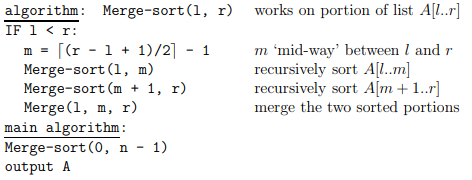
\includegraphics[scale=0.7]{merge1}
\end{center}
\newpage
\subsection{Merging in merge sort}
We use an additional workspace to merge our two halved in the form of another list, B
\begin{lstlisting}[tabsize=4,mathescape]
algorithm: Merge(l, m, r)
leftptr = l and rightptr = m + 1
counter = l
WHILE leftptr $\leqslant$ m and rightptr $\leqslant$ r:
	IF A[leftptr] $\leqslant$ A[rightptr]:
		B[counter] = A[leftptr]
		leftptr = leftptr + 1
	ELSE:
		B[counter] = A[rightptr]
		rightptr = rightptr + 1
	counter = counter + 1
IF leftptr $\leqslant$ m:
	B[counter..r] = A[leftptr..m]
ELSE:
	B[counter..r] = A[rightptr..r]
A[l..r] := B[l..r]
\end{lstlisting}
\subsection{How merging works}
To refine $B[counter..r] = A[rightptr..r]$
\begin{lstlisting}[tabsize=4,mathescape]
WHILE rightptr $\leqslant$ r:
	B[counter] = A[rightptr]
	counter = counter + 1
	rightptr = rightptr + 1
\end{lstlisting}
and to refine $A[l..r] = B[l..r]$
\begin{lstlisting}[tabsize=4,mathescape]
i = l
WHILE i $\leqslant$ r:
	A[i] = B[i]
	i = i + 1
\end{lstlisting}
\section{Sorting in Parallel}
Are either bubble, selection or merge sort amenable to parallel implementation?
\begin{itemize}
	\item In bubble sort you could have each processor checking each pair of numbers. However as two processors would be accessing the same number, we would have to take care with mutual exclusion
	\item There is not an obvious way to make selection sort parallel
	\item In merge sort each half list could be sorted using distinct processors. But you would need to make sure the lists were sorted before merging
\end{itemize}
\section{Research Glimpses}
\subsection{Coding Theory - Question from question sheet on this will not be on the exam}
\begin{itemize}
	\item Data Compression
	\begin{itemize}
		\item The compression of data for more efficient transportation
	\end{itemize}
	\item Error Correction/Detection
	\begin{itemize}
		\item Add extra data to messages to cope with errors in transit
	\end{itemize}
	\item Network Coding
	\begin{itemize}
		\item Different messages can be combined in transit, but so that the receiver can retrieve the original messages
	\end{itemize}
	\item Predictive coding
	\begin{itemize}
		\item The recovery of incomplete electronically stored information for use in legal cases, using mathematical coding theory
	\end{itemize}
\end{itemize}
\subsection{Algorithms for massive data sets}
The increase in large data sets ha lead to new models for memory
\begin{itemize}
	\item \textbf{External Memory Model} - The bulk of the data lies in secondary storage
	\item \textbf{Streaming model} - Data can only be accessed sequentially, not randomly 
\end{itemize}
\section{Binary Search}
We can easily search for an item in a list by amending the inner while loop in selection sort:
\begin{lstlisting}[tabsize=4,mathescape]
i = 0 and found = false
WHILE (i $\leqslant$ n - 1) and (found == false):
	IF A[i] 6= x:
		i = i + 1
	ELSE:
		found = true
output i
\end{lstlisting}
\begin{itemize}
	\item Note that if x appears in the list then the first location i where it appears is the output; otherwise n is the output
	\item However this algorithm is more efficient if the list is sorted
	\item Binary search is designed so that it finds an item in an already sorted list
\end{itemize}
Method
\begin{itemize}
	\item Compare the desired item with the median item in the list
	\item If the median is x then we are done
	\item If the median is greater than x then x lies to the left of the list, if it appears at all
	\item Re-perform on the halved list
\end{itemize}
\subsection{Pseudocode}
\begin{lstlisting}[tabsize=4,mathescape]
algorithm: Binary-search
leftptr = 0 and rightptr = n - 1
WHILE leftptr $\leqslant$ rightptr:
	m = $\ceil*{(leftptr + rightptr)/2}$
	IF A[m] $>$ x:
		rightptr = m - 1
	ELSE:
		IF A[m] $<$ x:
			leftptr = m + 1
		ELSE:
			return m
return n
\end{lstlisting}
\subsection{Binary Search in Action}
\begin{itemize}
	\item Binary search can be changed into a recursive algorithm
\end{itemize}
\begin{lstlisting}[tabsize=4,mathescape]
algorithm: Rec-Binary-search(l, r)
m = $\ceil{(l + r)/2}$
IF A[m] == x:
	return m
ELSE:
	IF l == m:
	return n
ELSE:
	IF A[m] $>$ x:
		index = Rec-Binary-search(l, m - 1)
		return index
	ELSE:
		IF m $<$ r:
			index = Rec-Binary-search(m + 1, r)
			return index
		ELSE:
			return n
main algorithm:
index = Rec-Binary-search(0, n - 1)
output index
\end{lstlisting}
\section{String matching}
The string matching problem:
\begin{itemize}
	\item We are given a test string and a pattern string
	\item We want to find an occurrence of the pattern of the test (if there is one)
\end{itemize}
Method:
\begin{itemize}
	\item The text string is given as an input in the list T[0...n-1] and the pattern string in the list P[0...m-1]
	\item The algorithm starts with the pattern aligned against the first m symbols of T
	\item If matches output true
	\item If not move along one
	\item Repeat
	\item Always compare from the right
\end{itemize}
\subsection{Pseudocode}
\begin{lstlisting}[tabsize=4,mathescape]
algorithm: Naive-String-Match
pos = 0
WHILE pos $\leqslant$ n - m:
	j = m - 1
	WHILE (j $\geqslant$ 0) and (P[j] == T[pos + j]):
		j = j - 1
	IF j < 0:
		return pos
	ELSE:
		pos = pos + 1
return n
\end{lstlisting}
\subsection{Naive string matching in action}
The algorithm can be slightly modified to find all occurrences of the pattern in the text
\begin{lstlisting}[tabsize=4,mathescape,escapechar=£]
algorithm: Naive-String-Match
pos = 0
£\textcolor{red}{flag=false}£
WHILE pos $\leqslant$ n - m:
	j = m - 1
	WHILE (j $\geqslant$ 0) and (P[j] == T[pos + j]):
		j = j - 1
	IF j < 0:
		output pos
		£\textcolor{red}{flag=true}£
	pos = pos + 1
£\textcolor{red}{If flag==false:}£
	output n
\end{lstlisting}
\section{Boyer-Moore string matching}
The naive string matching performs more comparisons than needed, because there is unused extra information. Consider the example below:
\begin{center}
	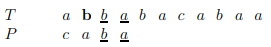
\includegraphics[scale=0.7]{Boyer-Moore}
\end{center}
\begin{itemize}
	\item We know that there are 2 matched symbols (\textbf{good suffix}) and a mismatched character, called the \textbf{bad character}
	\item Based on our knowledge of the good suffix and the pattern only, if we have the above mismatch, we can shift the pattern4 cells to the right. This is known as the \textbf{good suffix heuristic}
	\item Based on our knowledge of the bad character and the pattern only, if we have the above mismatch then we can shift the pattern 2 cells to the right before resuming. This is known as the \textbf{bad character heuristic}
\end{itemize}
\subsection{Modifying naive string matching}
\begin{itemize}
	\item Two functions, one for the good suffix, one for the bad character
	\item With good suffix, takes an input number and returns a number greater than zero, depending on the position you are in the string
	\item With bad character, take a letter from the alphabet, provide an offset
	\item Shift by maximum of good suffix and bad character
\end{itemize}
\section{Bioinformatics}
\begin{itemize}
	\item Take huge string of genetic characters and look for similarities to look at mutations and evolutions.
\end{itemize}


\end{document}